\subsection{Performance \& Model Size}\label{sec:disscusion:perf}

As seen in \Cref{section:eval}, \emph{wide Transformer networks typically offer equal or greater accuracy} on a range of classification tasks with different sequence lengths.
The impact of wider and shallower networks on accuracy is slightly influenced by the attention type, with some having more significant changes in accuracy than others.
There was no significant difference between convergence time during training for wide and deep models.
Each attention mechanism on each task achieved its best validation accuracy after roughly the same number of training steps for all model aspect ratios.

Whilst the total number of parameters involved in the attention layers remains constant amongst different aspect ratios, the overall number of parameters decreases.
This is due to the feed-forward network (FFN) part of the Transformer layer remaining unaltered as we change the models width.
The models with fewer layers have fewer FFN blocks, and so fewer parameters.

The deepest IMDb byte level classification and Listops models are typically 230MiB, with the widest models typically being 110MiB, only 48\% of the size.
On token level classification and document matching the sizes are closer.
Averaged across all tasks and attention mechanisms, the widest models are 71\% the size of the deepest models.
A full table of model sizes for the deepest and widest models across all tasks and attention types is given in \Cref{table:model_sizes}, in \Cref{appendix:model_size}.


\subsection{Latency}\label{sec:disscusion:lat}

As the number of layers in a model decrease, so does the number of dependencies in the computation graph.
Because of this a forward pass through the model will have lower latency, though overall throughput may remain unchanged.
For systems which require very low latency, such as real time processing in autonomous driving \citep{talpes2020compute}, this feature could make a wide single layer model more desirable than an equally accurate deep one.

We measure inference latency for the deepest and widest models for each task and attention type on a CPU with a single input, and on a GPU with a batch input.
Experimental details are given in \Cref{appendix:latency} along with raw numbers in \Cref{table:cpu_latency,table:gpu_latency}.
We find that on average the widest models are $3.1 \times$ faster on a CPU and $1.9 \times$ faster on a GPU than the deepest models.
The speed-up is consistent across all tasks and attention types.


\subsection{Interpretability}\label{sec:disscusion:interp}

\begin{figure}[hbt]
    \centering
    \begin{subfigure}{.35\textwidth}
        \centering
        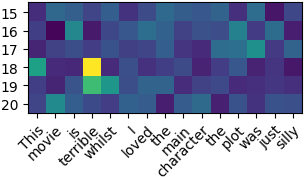
\includegraphics[height=0.12\textheight]{imgs/example_1_cropped.png}
        \caption{Prediction: strongly negative}
        \label{fig:wide_attention_1}
    \end{subfigure}
    \hspace{.05\textwidth}
    \begin{subfigure}{.55\textwidth}
        \centering
        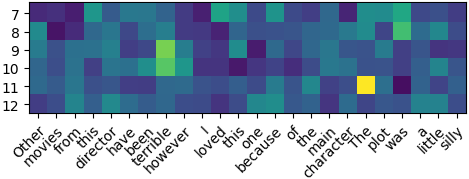
\includegraphics[height=0.12\textheight]{imgs/example_2_cropped.png}
        \caption{Prediction: weakly positive}
        \label{fig:wide_attention_2}
    \end{subfigure}
    \caption{The attention weights across a selection of heads with predicted classification for the single layer IMDb token level text classification Transformer model on two unseen and similar examples.}
    \label{fig:wide_attention}
\end{figure}

Interpretability is increasingly important and a very active area of machine learning research \citep{interpret1, interpret2}, especially when it comes to fairness.
By having more easily inspect-able models, we can see the reasons for a given classification.
For example, was a decision based on the mention of a protected characteristic, such as race or gender?

In a Transformer-based architecture, the attention heads in a layer can be inspected during inference to see what connections between input features that head found important.
For deep networks, many layers means it can often become unclear what the final output was actually based on \citep{tfm_interpret}.
For a single layer wide network, interpretability is far easier as only one layer needs to be inspected.
Thus what was considered important for the final output is much clearer.

In \Cref{fig:wide_attention}, we can see the attention weights across some of the heads of the widest token level text classification Transformer model, as well as the predicted class for two different example inputs that have been designed to be similar.
\Cref{fig:wide_attention} includes a subset of the total number of heads, for all 48 heads see \Cref{fig:wide_attention_full} in \Cref{appendix:attention}.

We can see the review on the left has been confidently assigned as a negative review, and from the attention weights we can see that this is due to the model recognising the relevance of the word ``terrible".
The review on the right has been less confidently assigned as positive.
From the attention weights we can see it has recognised words such as ``terrible", but the largest weight is on ``The". This explains why the model might not be confident in its positive prediction because it hasn't realised the importance of the word ``loved".


\subsection{Theoretical Explanations of Outliers}\label{sec:theory}

Most attention mechanisms usually have up to a 0.5\% increase in accuracy when going wider with two notable exceptions.
Longformer \citep{longformer} typically performs significantly better when deep, and Sinkhorn \citep{sinkhorn} typically performs significantly better when wide.

For Longformer we only use sliding window attention, with a width of 512.
This means, particularly for the longer tasks, each input feature can only have attention computed between it and its neighbours.
For deeper models, features can propagate and so this limitation is reduced.
However, single layer models suffers a performance penalty.

Sinkhorn works similarly to local attention, where the input sequence is divided into blocks.
Unlike local attention, which computes attention within these blocks, Sinkhorn sorts them and computes attention between the original block and the newly sorted block.
This sorting mechanism is learn-able per head., thus each head can learn a different sorting strategy.
For lots of heads this maximises the overall chance of important long range connections within the input sequence being attended to.


\subsection{Vision Transformer}\label{sec:discussion:vit}

There is a growing interest in applying Transformers to computer vision \citep{wang2021pyramid,wang2022pvt,liu2021swin,dosovitskiy2020image}.
We tested the Pyramid Vision Transformer model (PVT-V2-B1) \citep{wang2022pvt} and its wider variants on the CIFAR10 dataset \citep{krizhevsky2014cifar}.
The PVT-V2-B1 model has four stages with each stage containing two attention layers.
We then replace the two attention layers at each stage with a single wide attention layer.
The detailed architecture of the PVT-V2-B1 model and its wider variants are shown in \Cref{tab:vit}.
The first wider variant (Wide) matches the total number of heads to the original PVT-V2-B1 model, whereas the later variant (Wide-V2) contains a larger embedding size and more heads.
This is a closer match to the original model in terms of the model size.

\begin{table*}[!h]
	\caption{
		Performance of the original Pyramid Vision Transformer (PVT) and its wider alternatives on the CIFAR10 dataset.
		The original model (PVTV2-B1) has 4 stages, each stage contains two attention layers.
		((1, 1), (2, 2), (5, 5), (8, 8)) describes the original model,
		for instance, the first block contains two layers with a single head each, represented as (1, 1).}
	\centering
	\begin{tabular}{c|ccc}
	\toprule
	\textbf{Name}
	& \textbf{Configuration}
	& \textbf{Accuracy}
	& \textbf{Parameters} \\
	\midrule
	Baseline
	& $((1, 1), (2, 2), (5, 5), (8, 8))$
	& $95.59 \pm 0.99$	
	& $13.5$M	 \\
	Wide
	& $((2), (4), (10), (16))$
	& $94.54 \pm 0.31$	
	& $7.7$M	 \\
	Wide-V2
	& $((4), (8), (20), (32))$
	& $94.94 \pm 0.20$	
	& $12.6$M	 \\
	\bottomrule
	\end{tabular}
	\label{tab:vit}
\end{table*}


\Cref{tab:vit} illustrates that the wider variants do not outperform the original PVT-V2-B1 model.
Intuitively, spatial features play an important role in vision tasks.
The average pooling layer that comes before each attention layer is a crucial component of the PVT model.
With only a single wide layer, this pooling layer is not capturing as much spatial information as before.
The usage of a single wide attention layer in vision Transformers is constrained by the fact that the majority of these vision Transformers still use pooling or convolution layers before the attention.

